%\documentclass[12pt]{scrreprt}
\documentclass[12pt]{report}

\specialization{INFORMATICA}
\title{AI-Based Microjournaling for Self-Reflection using Emotion Detection and Clustering}
\author{Dumitrascu Constantin-Alexandru}
\supervisor{Professor, Lect. Horea Muresan}

\begin{document}

\maketitle

\newpage
\thispagestyle{empty}
\mbox{}
\newpage

\pagenumbering{roman}

\cleardoublepage
\begin{center}
\textbf{ABSTRACT}
\end{center}
\vspace{0.5cm}
\hrule
\vspace{0.5cm}

\begin{abstract}
This thesis presents the design, implementation, and empirical evaluation of GJournal, a privacy-first iOS microjournaling application that performs all natural language processing on the device. The system uses three interchangeable embedding strategies -- Apple NLEmbedding, all-MiniLM-L6-v2, and nomic-embed-text-v1.5 -- combined with adaptive DBSCAN clustering and a MobileBERT-based emotion classifier, all running locally via Core ML without any cloud component.

A central contribution is an empirical study of Matryoshka Representation Learning (MRL) applied to on-device semantic clustering. Nomic-embed-text-v1.5 is pre-trained with MRL, which allows its 768-dimensional output to be truncated to smaller sizes at inference time without retraining. The evaluation covers STS-B Spearman correlation, TwentyNewsgroups clustering quality, and a domain validation on 100 manually labelled journal entries. The main finding is that 256-dimensional Nomic embeddings retain over 99.5\% of the Spearman correlation of the full-dimensional model, while MRL inference latency remains flat at approximately 20\,ms across all truncation levels. On the journal-domain clustering task, all-MiniLM-L6-v2 achieves V-measure 0.662 and ARI 0.520, outperforming Nomic at any dimension on clustering purity.

The contributions of this thesis are: a fully on-device NLP pipeline for reflective journaling; quantized transformer models converted and deployed via Core ML; an adaptive DBSCAN clustering strategy tailored for short personal entries; a privacy-first application architecture; and a systematic MRL dimension-versus-quality trade-off analysis relevant to memory-constrained mobile deployment.
\end{abstract}

\cleardoublepage
\tableofcontents
\cleardoublepage

\pagenumbering{arabic}

\chapter{Introduction}
\label{ch:introduction}

Personal journaling has evolved from simple note-taking into a practice supported by digital tools that encourage self-reflection and emotional awareness. Recent advances in mobile hardware and on-device machine learning now allow private analysis of personal text without cloud services. This thesis examines whether those capabilities can support regular journalers who want a clearer picture of their emotional patterns over time.

The project proposes a mobile microjournaling system that processes short user entries on the device using compact language models, emotion detection, and clustering. Semantic representations of journal entries are grouped by similarity to surface recurring themes and emotional trends not visible in a flat chronological list. All computation runs locally, so user text never leaves the device.

The methodology builds on prior work in emotion recognition on edge devices \cite{Pandelea2021EmotionEdge}, efficient clustering for mobile processors \cite{awad2022improved}, and NLP-assisted journaling systems \cite{10351450}. Compact transformer architectures such as MobileBERT \cite{sun2020mobilebert}, DistilBERT \cite{sanh2019distilbert}, and TinyBERT \cite{jiao2020tinybert} show that competitive language understanding is achievable at a fraction of full-size BERT's cost, well within the budget of a smartphone NPU.

A more recent development relevant to on-device deployment is Matryoshka Representation Learning (MRL) \cite{kusupati2022matryoshka}. MRL trains a model with a nested loss so that every prefix sub-vector of the output is itself a useful embedding. In practice this means a single model can produce vectors at multiple dimensionalities without retraining or recompression: a 768-dimensional output can be truncated to 256 or 128 dimensions at inference time. This thesis evaluates nomic-embed-text-v1.5 \cite{nussbaum2024nomic}, an MRL-trained model, alongside all-MiniLM-L6-v2 \cite{reimers2019sentencebert} and Apple's NLEmbedding, to understand whether MRL dimension flexibility translates into a practical trade-off for on-device journaling.

The central question this thesis investigates is: at what MRL truncation level does Nomic match all-MiniLM-L6-v2 on journal-entry clustering quality, and what does the dimension-versus-quality curve look like across standard and domain-specific benchmarks? The short answer, established in Chapter~\ref{chap:evaluation}, is that 256-dimensional Nomic embeddings retain nearly all of the Spearman correlation relative to the full 768-dimensional model, but MiniLM still leads on clustering V-measure when tested against actual journal entries.

The thesis is organised as follows. Chapter~\ref{ch:background} reviews related work on digital journaling, on-device NLP, sentence embedding models, MRL, and mobile hardware. Chapter~\ref{ch:requirements} specifies the functional and non-functional requirements for GJournal and defines the architecture. Chapter~\ref{ch:implementation} describes the implementation: the data model, AI pipeline, clustering algorithm, and user interface. Chapter~\ref{chap:evaluation} presents the empirical evaluation across four models on STS-B, TwentyNewsgroups clustering, domain validation, and an on-device efficiency benchmark. Chapter~\ref{conclusions} summarises the findings and outlines directions for future work.

\section*{Note on the use of generative AI}
During the preparation of this thesis, the author used Claude Opus to improve the language and readability of the written text and to improve the readability of the source code. After using Claude Opus, the author reviewed and edited the output as needed. All experimental results, model training, system design, evaluation, and scientific conclusions are entirely the author's own work. The author takes full responsibility for the accuracy and integrity of the final document and codebase.

\chapter{System Requirements and Specification}
\label{ch:requirements}
\section{Scope and Objectives}

The application targets iOS and performs all natural language processing on the device. It stores short journal entries locally, generates semantic embeddings and emotion labels for each entry, and groups entries into clusters shown in list, calendar, and graph views. No user text leaves the device. The minimum target hardware is iPhone 14.


\section{Assumptions and Constraints}
The following assumptions and constraints are used throughout the specification:
\begin{itemize}
  \item Target platform: iOS 26+.
  \item All NLP inference and clustering run on device; cloud sync is not supported.
  \item Entry length is limited to approximately 500--600 characters.
  \item Minimum supported device class: iPhone 14 or equivalent NPU capability.
  \item Development stack: Swift + SwiftUI, Core ML for inference, SwiftData for local persistence, Python (RTX2070) for model fine‑tuning and conversion.
  \item Models will be quantized and converted to Core ML format to reduce size and improve inference speed.
  \item Where user input is incomplete, reasonable defaults are chosen and documented in this chapter.
\end{itemize}

\section{Functional Requirements}

\subsection{Core Functionality}
\begin{description}
  \item[FR1] \textbf{Create micro‑journal entry.} The user can create a short text entry. The entry editor opens a focused input screen that "takes the story" from the user.
  \item[FR2] \textbf{Entry views.} The user can view entries in a calendar view, a chronological list view, and a graph view that visualizes clusters and relationships.
  \item[FR3] \textbf{On‑device analysis.} Immediately after saving an entry, the system generates a semantic embedding and runs an emotion classifier locally.
  \item[FR4] \textbf{Clustering.} The system groups entries into clusters using an on‑device clustering algorithm. Clustering runs incrementally on new entries and can be re‑computed in batch.
  \item[FR5] \textbf{Search and filtering.} The user can search entries by text and filter by date, detected emotion, and cluster membership.
\end{description}

\subsection{Editing and Deletion Policies}
\begin{description}
  \item[FR6] \textbf{Edit policy.} The user may edit entries created on the same calendar day. Edits update embeddings and cluster assignments.
  \item[FR7] \textbf{Deletion policy.} The user may delete entries. Deleted entries are soft‑deleted and retained for a configurable grace period (default three days) before permanent removal.
\end{description}

\section{Non‑Functional Requirements}
\begin{description}
  \item[NFR1] \textbf{Privacy.} No user text or embeddings leave the device. No cloud services are used for inference or storage.
  \item[NFR2] \textbf{Performance.} Interactive analysis latency should be under five seconds on the minimum target device for a single entry; background batch clustering may take longer.
  \item[NFR3] \textbf{Model footprint.} Individual on‑device models should be quantized and kept as small as practical. The default configuration (MiniLM + emotion classifier) occupies 144\,MB; the full bundle including the Nomic model adds 274\,MB.
  \item[NFR4] \textbf{Battery and resource usage.} Background processing must be scheduled to minimize battery impact; heavy tasks should run when the device is idle or charging.
  \item[NFR5] \textbf{Accessibility.} The UI must follow platform accessibility guidelines (dynamic type, VoiceOver support).
\end{description}

\section{System Architecture}

\subsection{Components}
The UI Layer (SwiftUI) covers the entry editor, calendar, list, graph, and settings screens. The Persistence Layer (SwiftData) is a local database for entries, embeddings, cluster metadata, and user settings. The Inference Engine (Core ML) loads and runs on‑device models for embedding generation and emotion classification. The Clustering Engine implements a density‑aware algorithm (DBSCAN or similar) optimized for small datasets and incremental updates. A Scheduler and Background Worker manages periodic batch clustering, model updates, and low‑priority maintenance tasks.

\subsection{Architecture Diagram}
\begin{figure}[h!]
  \centering
  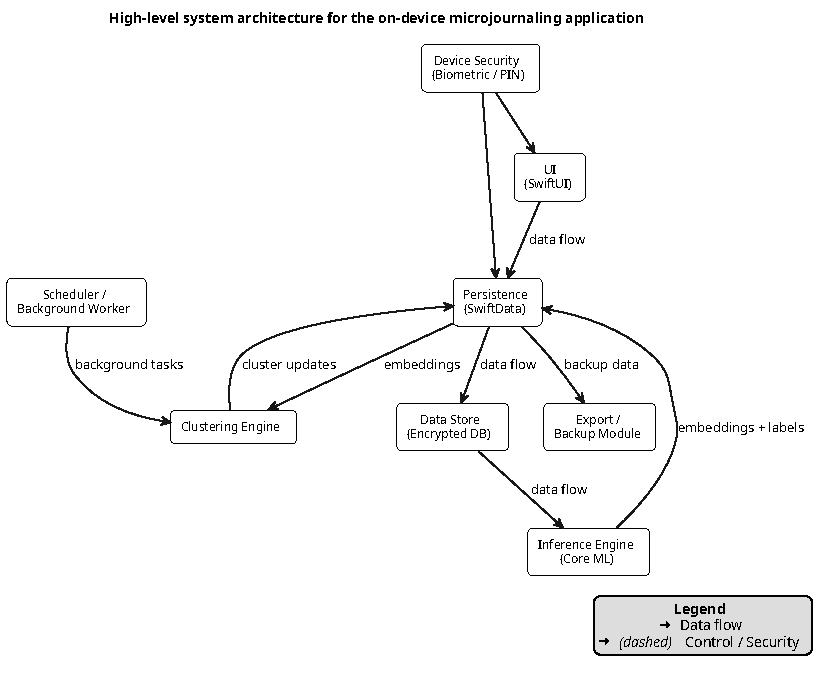
\includegraphics[width=0.85\textwidth]{figures/architecture.pdf}
  \caption{High‑level system architecture showing major components and data flow.}
  \label{fig:architecture}
\end{figure}

\section{Data Flow and Processing Pipeline}
The canonical data flow for a new entry is:

\begin{enumerate}
  \item User creates an entry in the editor and saves it.
  \item The Persistence Layer stores the raw text and metadata.
  \item The Inference Engine generates a semantic embedding and an emotion label for the entry.
  \item The embedding and label are stored alongside the entry.
  \item The Clustering Engine performs an incremental update to cluster assignments.
  \item The UI updates calendar, list, and graph views to reflect the new entry and cluster membership.
\end{enumerate}

A periodic batch job re‑computes clusters and cluster summaries during idle time or when the device is charging.

\section{Use Cases and User Flows}

Table~\ref{tab:use_cases} summarises the four primary use cases.

\begin{table}[h!]
\centering
\caption{Primary use cases.}
\label{tab:use_cases}
\begin{tabular}{p{0.14\textwidth} p{0.30\textwidth} p{0.44\textwidth}}
\hline
\textbf{Use Case} & \textbf{Trigger} & \textbf{System Response} \\
\hline
UC1 Create Entry &
  User fills in Feel, Event, and Action fields and taps Save &
  Entry stored; embedding and emotion label generated on device; cluster assignments updated; calendar, list, and graph views refreshed. \\
\hline
UC2 View Insights &
  User opens the Graph or Insights screen &
  Clusters shown with representative entries and emotion distribution. Tapping a cluster reveals its members. \\
\hline
UC3 Edit Entry &
  User edits an entry created on the same calendar day &
  Text updated; embedding and emotion label recomputed; cluster membership reassigned. \\
\hline
UC4 Delete Entry &
  User deletes an entry &
  Entry soft-deleted and hidden immediately; permanently removed after the three-day grace period. \\
\hline
\end{tabular}
\end{table}

\section{Model Selection and Formats}
Three embedding strategies are implemented behind a common \texttt{EmbeddingService} protocol. all-MiniLM-L6-v2 produces 384-dimensional mean-pooled embeddings and is packaged as a 45\,MB Core ML bundle; it is the default. nomic-embed-text-v1.5 is trained with Matryoshka Representation Learning and produces embeddings at \{64, 128, 256, 512, 768\} dimensions by truncating its output; the default truncation is 256 dimensions and the Core ML package is 274\,MB. Apple NLEmbedding ships with the operating system (zero bundle cost) and produces 512-dimensional vectors. The emotion classifier is MobileBERT fine-tuned for three epochs on GoEmotions, with 28 original labels collapsed to 12 classes (Joy, Sadness, Anger, Fear, Love, Surprise, Disgust, Anxiety, Excitement, Gratitude, Hope, Guilt), packaged as a 99\,MB Core ML bundle. All models are converted using coremltools on a Python workstation.

\section{Clustering Strategy}
The system uses DBSCAN with adaptive parameters. Epsilon is calibrated per corpus as the 10th percentile of pairwise cosine distances; \texttt{minPoints} scales with corpus size between a minimum of 3 and a maximum of 11. For MRL-truncated embeddings, epsilon is further scaled by $\sqrt{d/768}$ to compensate for the compressed distance range at lower dimensions. Each cluster is named by extracting frequent nouns and adjectives from its member entries; if no clear content words emerge, the dominant emotion label is used instead. A background batch job re-runs clustering when the device is idle.

\section{Privacy}
By design, the app does not transmit journal text, embeddings, or cluster metadata off device. No cloud services are involved in any part of the pipeline.

\section{Performance Targets and Testing}
Interactive inference (embedding + emotion classification) should complete within 5 seconds on iPhone 14; incremental cluster membership updates should complete within 2 seconds per new entry. Batch re‑clustering is acceptable to run for several minutes during idle or charging periods. The default model bundle (MiniLM + emotion classifier) targets under 200 MB; the optional Nomic model adds a further 274 MB. The journal database should remain responsive up to 200 MB of stored entries. Testing covers latency, memory, and battery impact on representative devices (iPhone 14 Plus, iPhone 15), and clustering quality via silhouette and ARI metrics on synthetic and anonymized sample data.

\section{Acceptance Criteria}
The prototype is acceptable when FR1--FR7 are implemented and demonstrable, on‑device inference meets the performance targets on the minimum device, data remains local with no off-device transmission, and clustering produces coherent groups visible in the graph view.

\section{Implementation Milestones}
The prototype was developed in five stages:
\begin{enumerate}
  \item \textbf{Scaffolding:} SwiftUI screens for the editor, calendar, list, graph, and settings; SwiftData schema for \texttt{Bit} and \texttt{Cluster} entities.
  \item \textbf{AI pipeline:} Core ML integration for all-MiniLM-L6-v2, nomic-embed-text-v1.5 MRL, Apple NLEmbedding, and MobileBERT emotion classifier; protocol-based \texttt{EmbeddingService} and \texttt{EmotionService} abstractions for interchangeable backends.
  \item \textbf{Clustering engine:} adaptive DBSCAN with epsilon calibration, incremental update on entry save, background batch re-clustering, and TF-IDF cluster naming.
  \item \textbf{Graph visualisation:} force-directed layout, hub-and-spoke edge rendering, pan/zoom gesture handling.
  \item \textbf{Evaluation:} Python benchmarks on STS-B and TwentyNewsgroups; domain validation on 100 labelled journal entries; on-device efficiency benchmark via an in-app measurement tool.
\end{enumerate}

\section{Traceability Matrix}

\begin{table}[h!]
\centering
\caption{Requirement traceability.}
\label{tab:traceability}
\begin{tabular}{p{0.16\textwidth} p{0.36\textwidth} p{0.34\textwidth}}
\hline
\textbf{Requirement} & \textbf{Implementation Component} & \textbf{Acceptance Test} \\
\hline
FR1 Create entry      & SwiftUI editor, SwiftData \texttt{Bit} model          & Save entry; verify text stored and visible in calendar \\
FR2 Entry views       & Calendar, list, graph SwiftUI screens                  & New entry appears in all three views after save \\
FR3 On‑device analysis & \texttt{AIProcessingManager}, Core ML services         & Embedding and emotion label present on \texttt{Bit} after save \\
FR4 Clustering        & \texttt{DBSCANClusterer}, \texttt{Cluster} model        & Entry assigned to cluster; cluster visible in graph \\
FR5 Search/filter     & Repository search API, filter chips                    & Filtering by emotion and cluster returns correct entries \\
FR6 Edit policy       & Editor day-lock logic, embedding update                & Edit updates text, re-runs inference, reassigns cluster \\
FR7 Deletion          & Soft-delete flag, maintenance pass                     & Deleted entry hidden immediately; removed after grace period \\
\hline
\end{tabular}
\end{table}

\section{Open Issues}
The main open issue is SwiftData schema migration: the current implementation wipes stored data on model changes during development. A versioned migration policy is required before any production deployment.

\section{Summary}
This chapter specified the functional and non‑functional requirements, the high‑level architecture, data flow, and acceptance criteria for the on‑device microjournaling system. The next chapter will describe the implementation details, model conversion steps, and the evaluation methodology used to validate the prototype.

\chapter{Design, Implementation, and Testing}
\label{ch:implementation}

This chapter presents a concise, implementation‑focused version of the design, data model, AI pipeline, clustering, visualization, and the functional test (F1) for the GJournal prototype.

\section{Scope and Objectives}
The prototype targets iOS/iPadOS/macOS and performs all NLP on device. Objectives:
\begin{itemize}
  \item Secure, local micro‑journaling with short entries.
  \item On‑device embedding and emotion detection per entry.
  \item Semantic grouping (clusters) and presentation via list, calendar, and graph.
  \item Preserve privacy: no cloud inference or storage.
  \item Maintain interactive performance on devices from iPhone 11 onward.
\end{itemize}

\section{High‑level Architecture}
GJournal uses a four‑layer architecture: \textbf{UI (SwiftUI)}, \textbf{Repository}, \textbf{Service} (AIProcessingManager, DBSCANClusterer, SafetyFilter), and \textbf{Persistence (SwiftData)}. Services are injected via protocol interfaces so mock implementations can be replaced by Core ML models without changing higher layers.

\section{Data Model}
\texttt{SwiftData} stores the primary entities:

\subsection{Bit}
Essential fields:
\begin{itemize}
  \item \texttt{id, title, feel, event, action, createdAt, lastModified}
  \item User selections: \texttt{feelEmotionRawValue, eventEmotionRawValue, actionEmotionRawValue, intensity}
  \item AI outputs: \texttt{embeddingJSON} (variable-length float array; 384 floats for MiniLM, 256 for Nomic-MRL default), \texttt{emotionProbabilitiesJSON}
  \item Flags/timestamps: \texttt{isHidden, isSafeContent, deletedAt, embeddingGeneratedAt, clusterAssignedAt}
  \item Computed accessors decode/encode JSON to typed arrays.
\end{itemize}

\subsection{Cluster}
Relational model with \texttt{@Relationship(deleteRule:.nullify)} to \texttt{Bit}. Cluster rows store \texttt{id, name, createdAt} and a list of member bits; names are updated centrally and observed reactively by SwiftData.

\subsection{Retention}
Soft delete sets \texttt{deletedAt}; a maintenance pass permanently removes entries after three days.

\section{Repository and UI Synchronization}
A repository pattern centralizes queries and writes. The repository exposes a \texttt{@Published bits: [Bit]} array; the AI pipeline sets a completion callback that reloads bits on the main thread so SwiftUI views update reactively. Search APIs accept text, emotion, date range, intensity, and cluster filters.

\section{AI Processing Pipeline}
The \texttt{AIProcessingManager} runs a six‑step pipeline on a background task (utility priority):

\begin{enumerate}
  \item \textbf{Text flattening:} combine title, Feel, Event, Action into a tagged string for the model.
  \item \textbf{Safety filter:} on‑device keyword scan across harm categories; flagged entries are stored but excluded from clustering/recommendations.
  \item \textbf{Embedding:} produce a fixed-length vector using one of three interchangeable services behind the \texttt{EmbeddingService} protocol: \texttt{CoreMLEmbeddingService} (all-MiniLM-L6-v2, 384-dim, mean pooling, 43\,MB Core ML package), \texttt{NomicEmbeddingService} (nomic-embed-text-v1.5 with MRL truncation, default 256-dim, 261\,MB Core ML package), or \texttt{NLEmbeddingService} (Apple's built-in \texttt{NLEmbedding}, 512-dim, zero bundle cost). \texttt{ServiceContainer} selects which service to wire via the \texttt{EmbeddingModelChoice} enum.
  \item \textbf{Emotion detection:} probability distribution over 12 emotion classes, produced by \texttt{CoreMLEmotionService}: MobileBERT fine-tuned on GoEmotions (28 labels collapsed to 12), converted to a 94\,MB Core ML package. Classes: Joy, Sadness, Anger, Fear, Love, Surprise, Disgust, Anxiety, Excitement, Gratitude, Hope, Guilt.
  \item \textbf{Persistence:} write embedding, emotion probabilities, safety flag, and timestamps on the MainActor.
  \item \textbf{Clustering:} re‑run DBSCAN and update \texttt{Cluster} rows.
\end{enumerate}

The pipeline minimizes UI latency by running off the main thread and switching to the MainActor only for persistence.

\section{Clustering}
\begin{itemize}
  \item \textbf{Algorithm:} DBSCAN chosen for no required cluster count and noise detection.
  \item \textbf{Distance:} cosine distance \(d(a,b)=1-\frac{a\cdot b}{\|a\|\|b\|}\).
  \item \textbf{Parameters:} adaptive epsilon calibrated per corpus via \texttt{calibrate\_epsilon} (10th percentile of pairwise distances); adaptive \texttt{minPoints} scaled by corpus size (minimum 3, maximum 11). For MRL-truncated embeddings, epsilon is further scaled by $\sqrt{d / 768}$ to compensate for the compressed distance range at lower dimensions.
  \item \textbf{Naming:} NLP-based namer extracts frequent nouns/adjectives from cluster entries; fallback to dominant emotion.
  \item \textbf{Complexity:} pairwise distance matrix \(O(N^2)\) acceptable for hundreds of entries; future optimizations (indexing/approximate NN) planned for scale.
\end{itemize}

\section{Knowledge Graph Visualization}
\begin{itemize}
  \item \textbf{Layout:} force‑directed simulation with global repulsion, intra‑cluster attraction (hub‑and‑spoke), and cluster gravity.
  \item \textbf{Initialization:} cluster‑aware sector placement to speed convergence.
  \item \textbf{Rendering:} hub‑and‑spoke edges to reduce edge count to \(O(N)\) per cluster.
  \item \textbf{Interaction:} pan, pinch‑to‑zoom, draggable nodes, and detail cards; gesture layer attached to a fixed clear background to avoid dead zones.
\end{itemize}

\section{User Interface}
Key screens and features:
\begin{itemize}
  \item \textbf{Dashboard:} greeting, activity heatmap, top emotions, quick entry.
  \item \textbf{Editor:} Feel–Event–Action fields, emotion wheel, intensity picker, auto‑save drafts.
  \item \textbf{List and Calendar:} grouped entries, full‑text search, emotion and cluster filter chips, sorting.
  \item \textbf{Graph:} interactive cluster graph with centroid labels and node detail cards.
\end{itemize}

\section{Dependency Injection and Testability}
All AI services are protocol‑based and provided by a \texttt{ServiceContainer} with three configurations: \texttt{makeMock()} (development), mixed device testing, and \texttt{makeProduction()} (Core ML models). This enables unit testing and device testing without changing application logic.

\section{Functional Test F1}
\textbf{Scope:} FR2 (create entry), FR4 (on‑device analysis), FR5 (clustering).  
\textbf{Procedure:} create a Bit in the editor, save, observe console logs, and verify calendar, list filters, and graph.  
\textbf{Expected / Observed:}
\begin{itemize}
  \item Entry persisted immediately and visible in calendar.
  \item Pipeline logs show steps 1–6; mock embedding generated (200\,ms delay).
  \item Clustering completed within seconds for small corpus; cluster name generated and filter chip appears.
  \item Knowledge graph shows the new node after clustering.
\end{itemize}

\section{Limitations and Next Steps}
\begin{itemize}
  \item Schema migration: SwiftData currently wipes the store on model changes during development. A versioned migration policy is needed before production deployment.
  \item Accessibility: VoiceOver labels on graph nodes and emotion-wheel controls require a dedicated pass.
  \item Notification rules: the scheduler logic for daily journaling reminders is defined but the exact trigger conditions (time window, streak rules) are not yet finalised.
  \item Keychain security: embedding vectors and emotion data are stored in SwiftData; a Keychain-backed encryption layer for the database file is planned.
\end{itemize}

\section{Acceptance Criteria (for this chapter)}
The implementation described here is acceptable when:
\begin{itemize}
  \item F1 is demonstrable: entry creation triggers the full pipeline and updates UI views.
  \item Data remains local and encrypted; biometric/PIN gating functions in device builds.
  \item Clustering and naming produce coherent groups on a sample dataset.
  \item Performance targets (interactive latency, incremental clustering) are met or have a documented mitigation plan.
\end{itemize}

\section{Summary}
This chapter presents the design, data model, AI pipeline, clustering algorithm, and functional test for the GJournal prototype. The system runs three interchangeable embedding services and a 12-class emotion classifier entirely on device. Remaining work is operational rather than architectural: schema migration, accessibility, and notification rules.

\chapter{Evaluation}
\label{chap:evaluation}

\section{Evaluation Setup}

\subsection{Datasets}

Two standard datasets cover different aspects of embedding quality:

\begin{itemize}
  \item \textbf{STS-B} (Semantic Textual Similarity Benchmark): 1500 sentence pairs scored by human annotators on a 0--5 similarity scale. Spearman rank correlation between model-predicted cosine similarities and the gold scores measures how well a model captures semantic meaning.
  \item \textbf{TwentyNewsgroupsClustering}: 1000 sentences drawn from 20 newsgroup topic categories. Ground-truth topic labels allow direct measurement of clustering quality.
\end{itemize}

Domain validation uses 100 manually labelled journal entries written during the testing period, annotated with ground-truth topic groupings. This set tests whether behaviour on standard benchmarks carries over to the actual application domain.

\subsection{Metrics}

Embedding quality is measured with Spearman rank correlation ($r_s$) on STS-B. Clustering quality uses:

\begin{itemize}
  \item \textbf{V-measure}: harmonic mean of homogeneity and completeness. A cluster has high homogeneity if it contains entries from only one ground-truth class; high completeness if all members of a class land in the same cluster.
  \item \textbf{ARI} (Adjusted Rand Index): agreement between predicted clusters and ground-truth labels, corrected for chance. Values range from 0 (random) to 1 (perfect).
  \item \textbf{Noise fraction}: the share of points DBSCAN marks as noise and leaves unclustered. High noise can mean over-strict parameters or genuinely sparse embeddings.
\end{itemize}

\subsection{Hardware}

All Python benchmarks run on an Apple M-series processor using the MPS backend (PyTorch). Apple NLEmbedding embeddings are generated by a standalone Swift script (\texttt{embed\_apple\_nlp.swift}) running on the same machine via \texttt{swift} command-line, then consumed by the Python pipeline as pre-computed JSON. This approach is necessary because \texttt{NLEmbedding} is a macOS/iOS SDK API not accessible from Python.

\section{Embedding Models}

Three strategies are implemented in GJournal behind the \texttt{EmbeddingService} protocol:

\begin{itemize}
  \item \textbf{Apple NLEmbedding}: the sentence embedding provided by the iOS \texttt{NaturalLanguage} framework via \texttt{NLEmbedding.sentenceEmbedding(for: .english)}. It produces 512-dimensional vectors with no additional bundle cost; the model weights are part of the operating system. Because this API is only callable from Swift, a standalone macOS Swift script (\texttt{embed\_apple\_nlp.swift}) was written to embed all benchmark sentences and export them to JSON for the Python evaluation pipeline. This approach allowed Apple NLEmbedding to participate in all three evaluation steps under the same metrics and DBSCAN configuration used for the other models.
  \item \textbf{all-MiniLM-L6-v2} \cite{reimers2019sentencebert}: a 6-layer MiniLM model producing 384-dimensional mean-pooled embeddings. Converted to a 43\,MB Core ML package. This model is the default in GJournal.
  \item \textbf{nomic-embed-text-v1.5} \cite{nussbaum2024nomic}: a 768-dimensional model trained with Matryoshka Representation Learning (Section~\ref{sec:mrl}). Converted to a 261\,MB Core ML package. Each input requires the prefix \texttt{"clustering: "}. The GJournal default configuration uses 256-dimensional MRL truncation.
\end{itemize}

\section{Matryoshka Representation Learning}
\label{sec:mrl}

Standard embedding models fix output dimensionality at training time. Reducing it after training typically requires retraining from scratch or post-hoc compression, both of which degrade quality. Matryoshka Representation Learning \cite{kusupati2022matryoshka} avoids this by training the model with a nested loss: the full $d$-dimensional output optimises a similarity objective, and simultaneously each prefix sub-vector of length $d' < d$ optimises the same objective independently. The result is that any prefix of the output vector is itself a competitive embedding.

For GJournal, the practical consequence is that the 261\,MB nomic model can produce embeddings at \{64, 128, 256, 512, 768\} dimensions by truncating its output after inference. No additional models or fine-tuning are needed. Table~\ref{tab:mrl_tradeoff} shows how Spearman correlation, silhouette score, and latency change across dimensions.

\begin{table}[h]
\centering
\caption{Nomic-v1.5 MRL dimension trade-off on STS-B (clustering prefix)}
\label{tab:mrl_tradeoff}
\begin{tabular}{|r|c|c|c|c|}
\hline
\textbf{Dim} & \textbf{Spearman $r_s$} & \textbf{Silhouette} & \textbf{$\varepsilon$ (MRL-scaled)} & \textbf{Latency (ms)} \\
\hline
 64 & 0.8408 & 0.1193 & 0.0866 & 20.7 \\
128 & 0.8521 & 0.1122 & 0.1225 & 20.4 \\
256 & 0.8571 & 0.1004 & 0.1732 & 20.3 \\
512 & 0.8584 & 0.1097 & 0.2449 & 20.2 \\
768 & 0.8596 & 0.1158 & 0.3000 & 20.2 \\
\hline
\end{tabular}
\end{table}

Latency is flat across all dimensions: inference takes approximately 20\,ms regardless of output size because the transformer forward pass dominates and the output slice is cheap. The Spearman gap from 128-dim (0.8521) to full 768-dim (0.8596) is 0.0075, so the accuracy cost of $6\times$ compression is small. Quality drops more noticeably below 128 dimensions: going from 128 to 64 loses 0.0113 Spearman.

The scaled $\varepsilon$ column shows the DBSCAN neighbourhood radius after MRL adjustment: $\varepsilon_d = \varepsilon_{768} \cdot \sqrt{d / 768}$. This compensates for the fact that cosine distances in lower-dimensional spaces tend to be smaller on average, which would otherwise cause DBSCAN to over-cluster at short dimensions.

\section{Embedding Quality on STS-B}

Table~\ref{tab:embedding_quality} shows Spearman correlation on 1500 STS-B pairs.

\begin{table}[h]
\centering
\caption{Embedding quality on STS-B (1500 pairs, MPS device)}
\label{tab:embedding_quality}
\begin{tabular}{|l|c|c|}
\hline
\textbf{Model} & \textbf{Dim} & \textbf{Spearman $r_s$} \\
\hline
MiniLM-L6-v2      & 384 & \textbf{0.8672} \\
Nomic-v1.5        & 256 & 0.8403 \\
Nomic-v1.5        & 768 & 0.8447 \\
Apple NLEmbedding & 512 & 0.7171 \\
\hline
\end{tabular}
\end{table}

MiniLM leads by 0.023 over Nomic at full dimensionality. Increasing Nomic from 256 to 768 dimensions recovers 0.0044 Spearman, a marginal improvement that does not close the gap to MiniLM. Apple NLEmbedding scores 0.717, which is 0.150 below MiniLM and 0.127 below Nomic-768. The gap reflects the fact that Apple's on-device model is optimised for breadth of language tasks rather than semantic similarity specifically.

\section{Clustering Quality on TwentyNewsgroups}

Table~\ref{tab:clustering_quality} shows clustering metrics on 1000 TwentyNewsgroups sentences using adaptive DBSCAN, with epsilon calibrated to the 10th percentile of pairwise distances per model.

\begin{table}[h]
\centering
\caption{Clustering quality on TwentyNewsgroupsClustering (1000 sentences, adaptive DBSCAN)}
\label{tab:clustering_quality}
\begin{tabular}{|l|c|c|c|c|c|c|c|}
\hline
\textbf{Model} & \textbf{Dim} & \textbf{V-m} & \textbf{ARI} & \textbf{Homog} & \textbf{Compl} & \textbf{Noise\%} & \textbf{Clusters} \\
\hline
MiniLM-L6-v2      & 384 & \textbf{0.584} & \textbf{0.249} & 0.437 & 0.881 & 56.3\% & 6 \\
Nomic-v1.5        & 256 & 0.366          & 0.089          & 0.234 & 0.844 & 23.1\% & 3 \\
Nomic-v1.5        & 768 & 0.477          & 0.121          & 0.322 & 0.924 & 40.4\% & 5 \\
Apple NLEmbedding & 512 & 0.020          & 0.001          & 0.010 & 0.585 & 22.3\% & 2 \\
\hline
\end{tabular}
\end{table}

MiniLM achieves the best V-measure (0.584) and ARI (0.249). Its noise fraction is higher (56\%) because its tighter clusters leave borderline points unclaimed. Nomic-256 assigns 77\% of sentences to clusters but homogeneity drops to 0.23, meaning its clusters mix topics. Nomic-768 sits between the two on most metrics. Apple NLEmbedding collapses all 1000 sentences into 2 clusters with near-zero V-measure (0.020) and ARI (0.001). Its cosine-distance geometry at 512 dimensions is too flat for DBSCAN to find meaningful topic structure on this benchmark.

\section{Algorithm Comparison}

Four DBSCAN variants were compared on TwentyNewsgroups using Nomic-768 embeddings. Table~\ref{tab:algorithm_comparison} shows the results.

\begin{table}[h]
\centering
\caption{Algorithm comparison on TwentyNewsgroupsClustering (Nomic-768, 1000 sentences)}
\label{tab:algorithm_comparison}
\begin{tabular}{|l|c|c|c|c|c|c|}
\hline
\textbf{Algorithm} & \textbf{V-m} & \textbf{ARI} & \textbf{Homog} & \textbf{Compl} & \textbf{Noise\%} & \textbf{Clusters} \\
\hline
Vanilla DBSCAN   & 0.009          & 0.000          & 0.004          & 0.496 &  1.8\% &  2 \\
Classic Adaptive & 0.477          & 0.121          & 0.322          & 0.924 & 40.4\% &  5 \\
MRL-Adapted      & 0.183          & 0.017          & 0.106          & 0.685 & 27.2\% &  5 \\
HDBSCAN          & \textbf{0.737} & \textbf{0.421} & \textbf{0.832} & 0.661 & 63.3\% & 52 \\
\hline
\end{tabular}
\end{table}

Fixed-epsilon Vanilla DBSCAN collapses the corpus into two clusters regardless of topic, giving near-zero V-measure. Classic Adaptive, which calibrates epsilon per corpus, raises V-measure to 0.477. The MRL-Adapted variant scales epsilon by $\sqrt{d/768}$; on TwentyNewsgroups it underperforms Classic Adaptive (V-measure 0.183) because the uniform topic distribution does not benefit from the correction designed for short journal entries.

HDBSCAN achieves the best purity (V-measure 0.737, ARI 0.421) but produces 52 clusters on 1000 sentences. In a journaling app with 20 to 50 entries the equivalent behaviour would create a cluster per entry or small group, making the insight view uninformative. Classic Adaptive DBSCAN is the practical choice for this application.

\section{Domain Validation on Journal Entries}
\label{sec:domain_validation}

Table~\ref{tab:domain_validation} shows results on 100 manually labelled journal entries using adaptive DBSCAN.

\begin{table}[h]
\centering
\caption{Domain validation on 100 custom journal entries (adaptive DBSCAN)}
\label{tab:domain_validation}
\begin{tabular}{|l|c|c|c|c|c|c|}
\hline
\textbf{Model} & \textbf{V-m} & \textbf{ARI} & \textbf{Homog} & \textbf{Compl} & \textbf{Noise\%} & \textbf{Clusters} \\
\hline
MiniLM            & \textbf{0.662} & \textbf{0.520} & 0.552 & 0.828 & 30\% & 3 \\
Nomic-256         & 0.511          & 0.296          & 0.354 & 0.918 & 22\% & 2 \\
Nomic-768         & 0.481          & 0.253          & 0.327 & 0.909 & 12\% & 2 \\
Apple NLEmbedding & 0.459          & 0.369          & 0.339 & 0.711 & 56\% & 2 \\
\hline
\end{tabular}
\end{table}

On actual journal text the gap between MiniLM and Nomic widens. MiniLM V-measure is 0.662 versus 0.511 for Nomic-256, a difference of 15 percentage points. Nomic-768 has the lowest noise fraction (12\%), meaning it assigns the most entries to clusters, but homogeneity is only 0.327: many of those assignments group unrelated entries together. For a journaling app a cluster that mixes different topics will mislead the user more than leaving borderline entries unclustered. MiniLM's behaviour (tighter clusters with more noise) is the better fit here.

Apple NLEmbedding reaches V-measure 0.459 on the journal domain, ranking last among the four models. Its ARI (0.369) is higher than Nomic-256 (0.296) and Nomic-768 (0.253), which means its cluster assignments agree with the ground-truth groupings more than chance when points are actually clustered, but its 56\% noise fraction means more than half of entries are left unclustered entirely. The combination of low completeness (0.711) and high noise makes it unsuitable as the primary embedding model for a journaling application, though its zero bundle cost remains an advantage when storage is the binding constraint.

\section{Emotion Classification}
\label{sec:emotion}

The emotion classifier is MobileBERT \cite{sun2020mobilebert} fine-tuned for three epochs on GoEmotions \cite{demszky2020goemotions}, with 28 original labels collapsed to 12 classes: Joy, Sadness, Anger, Fear, Love, Surprise, Disgust, Anxiety, Excitement, Gratitude, Hope, and Guilt. The trained model was converted to a 94\,MB Core ML package.

Overall accuracy on the 4542-sample test set is \textbf{59.5\%}. Table~\ref{tab:emotion_results} shows per-class results sorted by F1.

\begin{table}[h]
\centering
\caption{Emotion classifier per-class results (MobileBERT, GoEmotions 12-class, 4542 test samples)}
\label{tab:emotion_results}
\begin{tabular}{|l|c|c|c|c|}
\hline
\textbf{Emotion} & \textbf{Precision} & \textbf{Recall} & \textbf{F1} & \textbf{Test samples} \\
\hline
Gratitude  & 0.748 & 0.892 & \textbf{0.813} & 352 \\
Love       & 0.745 & 0.597 & 0.663          & 960 \\
Anger      & 0.683 & 0.562 & 0.616          & 785 \\
Excitement & 0.525 & 0.711 & 0.604          & 387 \\
Fear       & 0.500 & 0.731 & 0.594          &  78 \\
Joy        & 0.653 & 0.514 & 0.576          & 803 \\
Guilt      & 0.482 & 0.710 & 0.574          &  93 \\
Sadness    & 0.485 & 0.524 & 0.504          & 313 \\
Disgust    & 0.363 & 0.667 & 0.470          & 123 \\
Surprise   & 0.514 & 0.426 & 0.466          & 439 \\
Hope       & 0.357 & 0.645 & 0.460          & 186 \\
Anxiety    & 0.306 & 0.478 & 0.373          &  23 \\
\hline
\end{tabular}
\end{table}

Performance varies across classes mostly because of dataset imbalance. Gratitude has 352 test samples and achieves F1 0.813; Anxiety has 23 samples and achieves F1 0.373. The model has not seen enough Anxiety examples to separate it reliably from adjacent classes like Fear and Sadness. For the journaling use case this trade-off is acceptable: Joy, Sadness, Anger, Love, and Gratitude account for the majority of everyday entries, and all of them score above F1 0.57. Rare-class misclassifications fall through to the keyword-based \texttt{SafetyFilter} as a fallback.

\section{Discussion}

MiniLM outperforms all other models on clustering metrics across both the standard benchmark and the journal domain. Its 384-dimensional output, trained for semantic similarity tasks, is better calibrated for cosine-distance DBSCAN on short texts. Nomic's MRL support does not close that gap.

Apple NLEmbedding scores 0.717 Spearman on STS-B, usable for rough semantic similarity but 0.15 below MiniLM. Its clustering performance is much weaker: V-measure 0.020 on TwentyNewsgroups and 0.459 on journal entries. The poor clustering result reflects the API's design: \texttt{NLEmbedding.sentenceEmbedding} is a general-purpose on-device model trained across many language tasks, not for dense retrieval or clustering. Its advantage is zero bundle cost; the weights ship with the OS. That makes it a reasonable fallback when storage is the binding constraint, but not the primary embedding strategy.

The MRL dimension table tells a different story for memory. Latency is flat at approximately 20\,ms regardless of dimension, so there is no speed benefit to using fewer dimensions. But storage is affected: at 256 dimensions each embedding occupies $256 \times 4 = 1024$ bytes versus $768 \times 4 = 3072$ bytes at full size. Over 1000 journal entries that is roughly 2\,MB saved in the SwiftData store. The Spearman cost of compressing from 768 to 256 dimensions is 0.0044, a drop of 0.52\%.

The practical outcome for GJournal is that MiniLM is the default: best clustering quality, smallest dedicated bundle at 43\,MB, no prefix requirement. Nomic at 256 dimensions is available as a user-selectable option where total model size must stay under a specific limit. Apple NLEmbedding remains available as a zero-cost fallback for devices where storage is the binding constraint.

\chapter{Concluzii}
\label{conclusions}

\par
The thesis considered the creation and execution of a privacy-preserving mobile microblogging platform capable of carrying out natural language processing computations right on the user’s smartphone. This research showed that using modern mobile computing hardware, specifically Neural Processing Units from iOS, iPadOS, and macOS, is a viable method to execute light-weight transformer-based computations for semantic embedding and emotion clustering.

\par
The architecture developed for this thesis manages to effectively combine quantized neural models, a safe method of local storage, and incremental clustering without having any personal information leave the device. Such an approach is highly important for the area of personal well-being apps because of its respect for privacy and confidentiality issues.

\par
The project provided technical evidence that transformers can be fine-tuned, compressed, and then run on consumer-grade mobile devices without sacrificing too much accuracy in the analysis of short-form texts. In addition, the clustering process showed that it is possible to gain valuable information from the micro-journals that can be displayed in calendar views, lists, or graphs.

\par
The following are the primary contributions made by this thesis: the design of a complete end-to-end NLP pipeline that runs entirely on-device, the implementation of quantized transformer architectures that can be executed on mobile devices, the creation of an incrementally clustering approach that is designed specifically for short entries by individuals, and finally, the design of a safe and privacy-centric application structure.

\par
Potential future directions include the enhancement of the emotion taxonomy, stabilization of the clustering process, inclusion of other modalities like speech and images, or cross-device encryption synchronization without compromising the security features. Regardless, the findings discussed in this thesis clearly demonstrate that on-device NLP is a viable approach to personal journaling applications.

\nocite{*}
\bibliography{references}

\end{document}
